\section{Support Vector Machine}

\subsection{Methods}
\subsubsection{Treatment of Data}
\paragraph{Splitting}
For the implementation of the SMO algorithm the training data had not to be split into fixed training and validation sets. Instead the imperative was to implement 10-fold crossvalidation for parameter selection of $\tau$ and C. In order to achieve this task and save time we used the KFold() method of the python scikit library. This method thus splits the dataset into 10 consecutive folds without shuffling. Each fold is then used once as a validation set while the k-1 remaining folds form the training set.
\paragraph{Preprocessing}
Regarding preprocessing we applied the same normalization as with the Multilayer Perceptron.

\subsubsection{SVM setup}
To determine the optimal parametrization of the SVM we ran the SMO algorithm with 10-fold crossvalidation for the following range of values of $C$ and $\tau$:
\begin{center}
\begin{tabular}{l|lllllllll} 
	\toprule
	$\tau$ & 0.002 & 0.004 & 0.008 & 0.016 & 0.032 & 0.064 & 0.128 & 0.256 \\
	C & 1 & 2 & 4 & 8 & 16 & 32 & 64 & 128 & 256 \\
	\bottomrule
\end{tabular}
\end{center}

\subsection{Results}
The resulting scores from the cross.validation are depicted in fig. \ref{fig:scores}. 
\begin{figure}[!ht]
	\centering
	\includegraphics[width=.7\textwidth]{svm/scores_max_300.eps}
	\caption{Summed up misclassification scores for range of parameters $C$ and $\tau$ depicted after 10-fold crossvalidation. The smallest total score 59 was recorded for $\tau=.128$ and $C=2$. The range of values is displayed up to a maximum score of 300 which represents 5\% misclassifications on the validation data over the 10 folds.}
	\label{fig:scores}
\end{figure}
\subsection{SVM criterion and Convergence criterion}
Through running the SMO with the two parameters found through cross-validation on the whole training set, we obtained the graphs for the SVM criterion\quad$\Phi$as a function of SMO iterations and the Convergence criterion $b_{up}-b_{low}$ based on KKT condition violations as shown in fig. \ref{fig:criterions}. Subfig. \ref{subfig:svm_criterion} clearly shows how $\Phi$ is minimized according to the support vector coefficients \textbf{$\alpha$}. The logarithmic scaling in subfig. \ref{subfig:logarithmic} shows us that the convergence criterion decreases near-exponentially through the course of the optimization.
\begin{figure}[!ht]
	\centering
	\begin{subfigure}[b]{.45\textwidth}
	\centering
	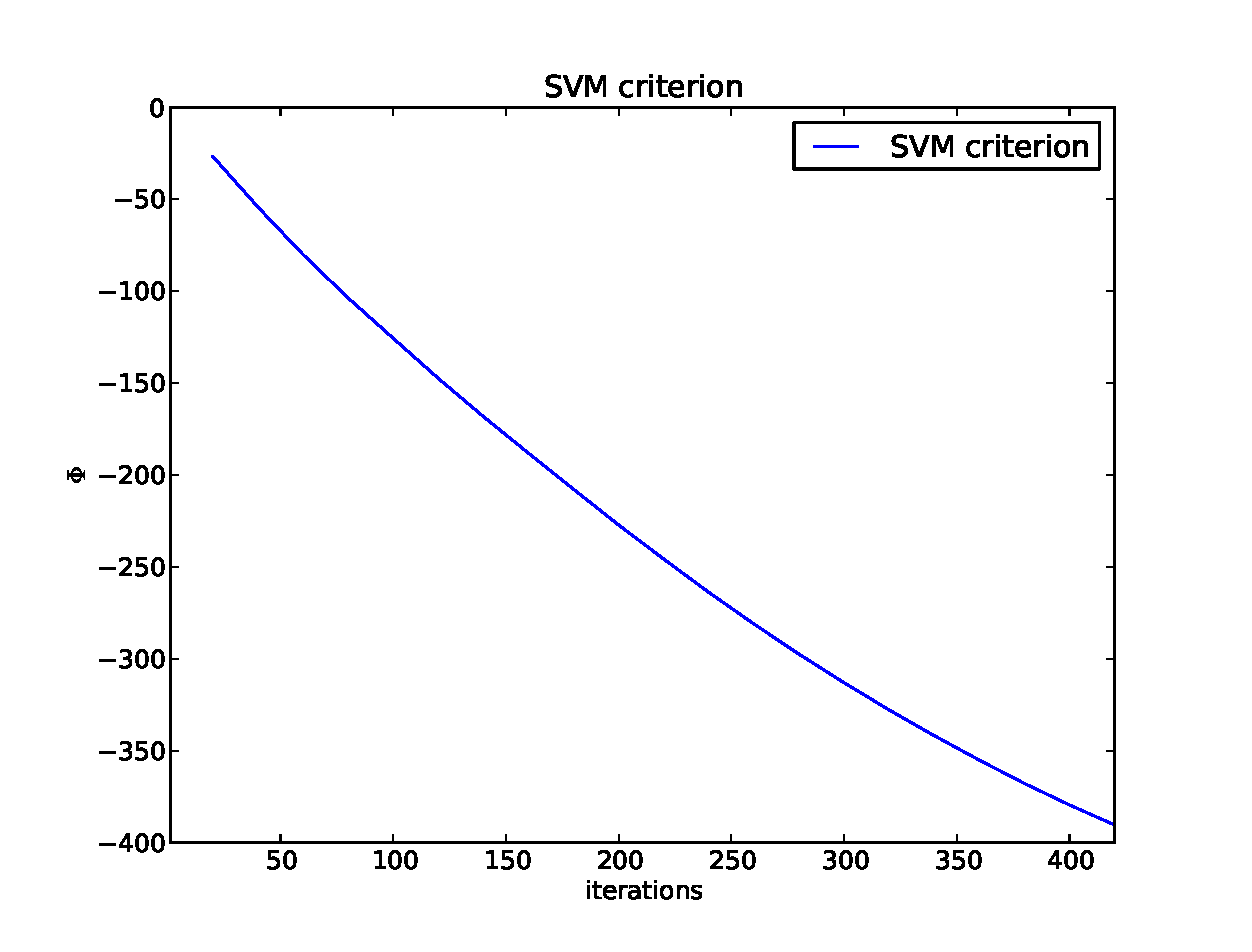
\includegraphics[width=\textwidth]{svm/svm_criterion.eps}
	\caption{SVM criterion $\Phi = \frac{1}{2}\sum_{i,j}\alpha_i\alpha_j t_i t_j -\sum_i \alpha_i$ over number of iterations}
	\label{subfig:svm_criterion}
	\end{subfigure}
	\quad
	\begin{subfigure}[b]{.45\textwidth}
	\centering
	\includegraphics[width=\textwidth]{svm/criterion_violations_plot.eps}
	\caption{Convergence criterion $f_i-f_j$ plotted over number of iterations of respective most violated pair}
	\label{subfig:logarithmic}
	\end{subfigure}
	\caption{SMO run on full training set with parameters found through cross-validation}
	\label{fig:criterions}
\end{figure}
\paragraph{SVM Performance}
Training with the SMO as discussed above results in a 0/1 training error of $0.0502\%$ and a classification error of $0.904\%$.

\subsubsection{Performance comparison of SVM and MLP}
In this section we make a comparison of the final setup of the Multilayer Perceptron and Support Vector Machine on the 4-9 classification problem. In fig. \ref{fig:comparison} we display the training and testing zero/one errors for the final parametrizations of the classification algorithms. One can see that SVM performs significantly better than the MLP, making less than 1\% wrong classifications. Both algorithms are of course powerful. Finding the optimal parameters for gradient descent of MLP may be faster than cross-validation for the SVM. However, the "kernel trick" makes nearly unbeatable in ways of complexity and fast setup, whereas changes in the architecture of the MLP can lead to different derivations of the gradient on the error function according to the weights of the network.
\begin{figure}[!ht]
	\centering
	\includegraphics[width=.7\textwidth]{svm/comparison_bar_plot.eps}
	\caption{Bar plot of 0/1 error for training and testing comparing final parametrizations MLP and SVM (including the standard deviation for the MLP)}	
	\label{fig:comparison}
\end{figure}